%----------------------------------------------------------------------------------------
\chapter{Analysis}
\label{chap:analysis}
%----------------------------------------------------------------------------------------

This chapter analyzes the problem of developing a \textbf{type-safe}
Domain-Specific Language for Alchemist simulations configuration. 
The analysis establishes the foundation for the design 
and implementation phases by identifying
requirements, constraints, and the domain model underlying the simulation configuration.


The chapter begins by defining the high-level goals for the DSL.
It then examines constraints that the solution must satisfy, 
including backward compatibility with the existing configuration system and 
limitations imposed by the \textbf{Kotlin} language.
Moreover, the requirements are defined and analyzed in more detail, including 
functional and non-functional requirements.

The analysis then investigates the limitations of the current YAML-based approach and examines 
how the existing type system constrains the solution. 
Finally, the chapter models the simulation configuration domain, 
identifying key concepts and their relationships that guide the DSL design.

\section{High-level Goals}

The \textbf{primary goal} is to develop a type-safe 
Domain-Specific Language in Kotlin that will replace YAML as the main configuration format for Alchemist simulations. 
The DSL should eliminate the type safety and tooling limitations of YAML 
while maintaining \textbf{semantic equivalence} with existing YAML configurations. 
The adoption of a \textit{Programming Language} for the simulation configuration should improve the 
overall developer experience and productivity:
the DSL can provide compile-time type and syntax checking, enabling early detection of configuration errors before simulation execution.
Moreover, the \textit{Integrated Development Environment} (IDE) support, including autocomplete and inline documentation, 
should reduce the learning curve and improve productivity when creating simulation configurations. 
The user can leverage the IDE to focus on the simulation configuration and less on the language syntax.

The \textbf{second goal} concerns compatibility and integration. 
The DSL must integrate seamlessly with Alchemist's existing loading infrastructure, 
producing identical simulation models to those generated from YAML. 
This ensures that simulations configured via the DSL behave identically to their YAML counterparts,
 preserving reproducibility and allowing gradual migration from YAML to the DSL.

The \textbf{third goal} focuses on expressiveness and maintainability. 
The DSL should provide a natural, domain-appropriate syntax that makes simulation configurations more readable and maintainable 
than their YAML equivalents. However, the DSL should have the same semantic as the YAML configuration, 
allowing the user to leverage their existing knowledge of YAML to configure simulations. Moreover, the DSL, 
should be open to extensions and should be able to support new features or new incarnations as they are developed, without 
the need to modify the DSL itself.


Next sections will analyze, in more detail, the constraints and functional requirements that the DSL must satisfy.
\section{Constraints}

Constraints define \textbf{limitations} and \textbf{conditions} that the DSL solution must satisfy, 
restricting the design space and implementation choices. 
These constraints arise from the need to integrate with existing systems and comply with language specifications.


Two primary constraint categories affect the DSL design:
\begin{itemize}
    \item \textbf{Backward compatibility}: ensures that the DSL integrates with Alchemist's 
    existing configuration system without breaking existing functionality. 
    \item \textbf{Language constraints}: the Kotlin language syntax and the available tooling capabilities 
    limit the implementation choices. 
\end{itemize}

These two constraints will be analyzed in more detail in the next sections.

\subsection{Backward Compatibility}
The backward compatibility constraint ensures that the DSL integrates with Alchemist's 
existing configuration system without breaking existing functionality. 
This constraint is crucial to ensure that the YAML configuration files can still be used to configure simulations, 
even after the DSL is adopted. The Kotlin DSL should be an \textbf{alternative} to YAML configuration format, not a replacement.
At the same time, the DSL should support all the existing YAML features and should be able to generate 
the same simulation model as the YAML configuration.

The development of the Kotlin DSL should not require any changes to the existing YAML configuration files.
The same is true for the\textit{ loading system }of Alchemist: 
it should be able to load both YAML and Kotlin DSL configuration files. 
The actual system should be extended but not replaced. 

\subsection{Kotlin Language Constraints}

Kotlin provides powerful DSL-building capabilities through receiver types and extension functions, 
enabling concise syntax for \textbf{builder} patterns. 
However, compared to languages like Scala, Kotlin imposes several constraints that affect DSL design and expressiveness.


Function naming restrictions limit DSL expressiveness. Kotlin requires function names to be valid identifiers, 
preventing the use of arbitrary symbols or special characters. 
While Kotlin supports infix functions and operator overloading, 
the set of overloadable operators is fixed and limited.
This restricts the ability to create domain-specific operators that might make configurations more intuitive.

Kotlin 1.6.20 introduced experimental context parameters as a mechanism for context-dependent declarations.
However, this feature remains experimental and has some limitations:  
context parameters cannot be used at class level or in constructors, 
restricting their applicability to property and function declarations only\footnote{\url{http://archive.today/twmFC}}.


\section{Functional Requirements}

Functional requirements specify what the DSL must accomplish to achieve the high-level goals 
while satisfying the identified constraints. 
These requirements define the essential capabilities and behaviors that the DSL implementation must provide.
Three primary functional requirements govern the DSL design:
\begin{itemize}
    \item \textbf{YAML equivalence}
    \item \textbf{Loading system integration}
    \item \textbf{Type safety}
\end{itemize}

These three functional requirements will be analyzed in more detail in the next sections.

\subsection{YAML Equivalence}
The YAML equivalence functional requirement ensures that the DSL can express all simulation configurations currently
representable in YAML and produces \textbf{identical} simulation models. 
Since it is assumed that the current YAML configuration system is working correctly,
it can be used as a reference to ensure that the DSL can produce the same simulation model. 
The Alchemist YAML specification can be used as a reference to define the semantic of the DSL, since we want 
the DSL to have the same semantic as the YAML configuration. 
The user should be, in theory, able to convert an existing YAML configuration file to a DSL configuration file and vice versa, 
and the two configurations should produce the same simulation model. Moreover, a user should expect 
to find in the DSL configuration system all the features of the YAML configuration system.


\subsection{Loading System Requirements}
The loading system requirements mandate integration with Alchemist's existing configuration 
loading infrastructure, enabling the DSL to work alongside YAML configurations.
The loading system should be able to load both YAML and Kotlin DSL configuration files. 
Currently, the loading system is able to load the simulation model from the YAML configuration file that is a
file with a \textit{.yaml} extension.
The loading system should be extended to be able to support also the new Kotlin DSL configuration file that is a
file with a \textit{.kts} extension. 
\begin{itemize}
    \item \textbf{Via Gradle}
    \item \textbf{Via Standalone Application}
\end{itemize}


\subsection{Type Safety}

Type safety represents a fundamental requirement for the DSL, addressing one of the most significant limitations 
of the YAML-based configuration approach. 
Unlike YAML, where configuration errors remain undetected until runtime,
the DSL must leverage Kotlin's type system to identify and report errors during development, before the simulation is executed.

The primary advantage of type safety lies in the immediate feedback it provides to developers. 
Modern IDEs can perform continuous type checking as the user writes code, 
highlighting errors in real-time through visual indicators such as red underlines and error messages. 
This immediate feedback transforms the development experience: instead of discovering a typo in a molecule name or an incorrect parameter
type only after running the simulation, developers receive instant notification that something is wrong. 
For instance, if a user attempts to assign a string value to a parameter that expects a numeric type, 
the IDE will immediately flag this as an error, preventing the mistake from propagating further into the development process.

Beyond error detection, type safety enforces a stricter interpretation of the configuration specification. 
The DSL's type system acts as a formal contract that constrains what constitutes valid syntax and structure. 
This enforcement mechanism guides developers toward correct configurations by making invalid constructs 
impossible to express within the type system. 
This contrasts sharply with YAML, where such structural requirements are only enforced through runtime validation.

Finally, the compile-time validation provided by type safety contributes to improved confidence in configuration correctness. 
Developers can trust that if their code compiles successfully, 
the configuration adheres to the type constraints, eliminating entire classes of syntax errors.
This feature should reduce the amount of time spent on fixing typos and other common errors in the configuration file.

\section{Non-functional Requirements}

While functional requirements define \textit{what} the DSL must accomplish,
 non-functional requirements specify \textit{how well} the system should perform 
 and what quality attributes it should exhibit. 

These requirements address the qualitative aspects of the DSL that determine its effectiveness, maintainability, 
and long-term viability. 
Non-functional requirements typically involve subjective assessments of quality, usability, and performance characteristics.

For a Domain-Specific Language, non-functional requirements play a crucial role in determining its adoption and success. 
A DSL that fulfills all functional requirements but is difficult to use, lacks extensibility,
 or performs poorly will likely fail to gain traction among developers. 
These requirements ensure that the DSL not only works correctly but also provides a
 positive user experience and can evolve to meet future needs.

 The next sections will analyze in more detail the non-functional requirements.

\subsection{DSL API Usability}

Usability is a critical quality attribute for a Domain-Specific Language, 
directly influencing its adoption and effectiveness.
For the Alchemist DSL, usability encompasses readability, learnability, and the ability to
 express complex configurations with clarity.
The API design must be rooted in the existing Alchemist domain model, 
using familiar concepts such as \textit{nodes}, \textit{molecules}, \textit{reactions}, 
and \textit{environments} as first-class syntax elements.
This semantic alignment ensures that users already familiar with the Alchemist 
ecosystem and its YAML syntax can transition to the DSL with minimal effort.
The DSL syntax should intuitively map to the mental model of the simulation, 
reducing the cognitive load required to translate a simulation design into code.
It should be easy for a user to switch to the new DSL syntax without
 needing to learn a completely new paradigm.

A key aspect of usability is the prevention of ambiguity and structural errors during 
configuration.
In Kotlin's type-safe builders, a common pitfall is \textit{scope leakage}, 
where members of an outer receiver remain accessible within nested blocks.
For example:
\begin{minted}[fontsize=\footnotesize]{kotlin}
html {
    head {
        head {} // should be forbidden
    }
    // ...
}
\end{minted}
\captionof{lstlisting}{Example of scope leakage in Kotlin}
To prevent such ambiguous constructions, the DSL must leverage the
 \texttt{@DslMarker}\footnote{\url{https://kotlinlang.org/docs/type-safe-builders.html\#scope-control-dslmarker}} annotation mechanism provided by Kotlin.
This annotation restricts implicit receiver access to the nearest scope,
 preventing the user from accessing outer receivers unless explicitly requested.
By strictly controlling scope visibility, 
the DSL guides the user towards valid structures and prevents 
common configuration errors at compile time.

Furthermore, the DSL structure should encourage readability by avoiding excessive nesting depth.
While hierarchical structures are natural for configuration, deep nesting can make files difficult to read and maintain.
The API should provide mechanisms to modularize configurations or define components concisely, resulting 
in cleaner and more readable files.

Finally, usability is heavily dependent on tooling support.
The DSL implementation must be designed to maximize the capabilities of modern IDEs and text editors.
This includes providing comprehensive documentation for all builder functions, which the IDE can display inline.
Features such as syntax highlighting, code navigation, and intelligent autocompletion 
are essential to guide the user through the configuration process,
 making the DSL not just a verification tool, but an active aid in simulation development.

\subsection{Extensibility}

Extensibility is a another fundamental quality attribute for the Alchemist DSL, 
given the framework's nature as a general-purpose simulator.
Alchemist is designed to be extended: users can define new \textit{incarnations}, 
implement custom \textit{reactions}, create specialized \textit{environments}, 
and introduce new data types for concentrations.
Consequently, the DSL must be equally extensible, capable of supporting both existing 
and future extensions without requiring modifications to the DSL core.

This requirement can be broken down into two key aspects: \textbf{modularity} and \textbf{openness}.

\paragraph{Modularity and Reusability}
The DSL must overcome the limitations of the current YAML configuration system regarding code reuse.
As analyzed in Chapter~\ref{chap:introduction}, YAML's reuse mechanisms are limited to file-local anchors,
 preventing the sharing of configuration components across multiple files.
The Kotlin DSL must allow users to define reusable simulation components, such as node templates, environment configurations, 
or reaction patterns, that can be imported and used in multiple simulation definitions.
This modularity should extend to the creation of \textbf{libraries}.
Advanced users should be able to package common configuration patterns 
(e.g., a library of standard crowd dynamics behaviors or a collection of biochemical reaction templates) 
and distribute them as dependencies.
This capability effectively transforms simulation configuration from writing monolithic
 files to composing simulations from well-tested, reusable building blocks.

\paragraph{Integration of New Functionalities}
The DSL design must align with Alchemist's open-closed principle.
When a user introduces a new feature into the simulator, for instance, 
a new \texttt{Incarnation} or a custom \texttt{TimeDistribution}, 
the DSL should be able to support it immediately.
Crucially, this support should not come at the cost of user experience.
Unlike the YAML approach, where extensibility is achieved by sacrificing type safety (via string-based class loading), 
the DSL must provide a mechanism to use these new components in a type-safe manner, 
ideally retaining IDE features like autocompletion and documentation.
This implies that the DSL architecture cannot rely on a hardcoded set of supported classes.
Instead, it requires a flexible integration strategy that can adapt to the user's classpath, 
bridging the gap between Alchemist's dynamic class loading and Kotlin's static type system.


\subsection{Performance}

In the context of this thesis, the performance requirement specifically refers to the efficiency 
of the \textbf{loading module} of Alchemist, that is the module responsible for the parsing of the configuration 
and the instantiation of the simulation model.
It is important to clarify that this requirement does not concern the runtime execution speed of the Alchemist simulation engine itself, 
as the internal simulation logic remains independent of the configuration format used.

While performance is a relevant quality attribute, it is prioritized lower than usability, type safety, and modularity.
The primary objective of the DSL is to improve the developer experience and the correctness of configurations.
Therefore, a slight overhead in the loading phase, typically associated with the compilation or evaluation of Kotlin scripts, 
is considered an acceptable trade-off for the benefits provided by a rich, strongly-typed language.

Nevertheless, the DSL implementation should strive to maintain performance levels comparable 
to the existing YAML-based loading system.
The loading process should remain efficient 
enough to support iterative development cycles where simulations are frequently reloaded.
Ideally, the solution should aim to match or potentially improve upon the current loading times,
 avoiding significant regressions that could hinder the user workflow.

 
\section{Requirements Analysis}

This section analyzes the implications of the previously described functional and non-functional requirements, 
identifying the core technical challenges that the design phase must address.
The primary challenge lies in reconciling the static nature of the DSL's type system with the flexible, 
dependency-rich instantiation model of the Alchemist simulator.

\subsection{The Challenge of Contextual Dependency Injection}
In a standard Kotlin program, instantiating a class requires providing arguments for all its constructor parameters.
However, Alchemist's model classes are designed to be instantiated via a dependency injection mechanism.
Their constructors often require two types of parameters:
\begin{itemize}
    \item \textbf{Configuration parameters}: Values that define the specific 
    behavior of the instance (e.g., the radius of a neighborhood, the probability of a reaction).
     These are the values the user intends to configure.
    \item \textbf{Contextual parameters}: Objects representing the simulation state or 
    services (e.g., \texttt{Environment}, \texttt{RandomGenerator}, \texttt{TimeDistribution}). 
    These are technical dependencies required for the object to function but are typically managed by the framework, not the user.
\end{itemize}

In the YAML loader, this distinction is handled dynamically: 
the system inspects the constructor, automatically injects the available contextual parameters,
 and asks the user only for the configuration parameters.
Transitioning to a static DSL poses a challenge: a direct constructor call in Kotlin would force the user to 
manually provide all parameters, including the contextual ones.
This would degrade usability, making the configuration verbose and exposing internal implementation details.

Therefore, the DSL must provide a mechanism to \textbf{bridge} this gap.
It needs to expose a simplified, declarative API where users specify only the configuration parameters, 
while the DSL implementation automatically resolves and injects the contextual dependencies.
Crucially, to satisfy the \textbf{Extensibility} requirement, this mechanism cannot be hardcoded for a fixed set of classes.
It must be general enough to support user-defined implementations, allowing them to benefit from the same 
auto-injection capabilities as built-in components without requiring significant boilerplate code.
This suggests the need for a generative approach to create these simplified APIs automatically.

\subsection{Prioritization of Quality Attributes}
Given the trade-offs involved, the analysis establishes the following hierarchy of quality attributes to guide design decisions:

\begin{enumerate}
    \item \textbf{Correctness and Safety}: The DSL must prevent invalid configurations.
     If a trade-off must be made between flexibility and safety, safety generally takes precedence. 
     However, the system must not prevent valid configurations that are possible in YAML.
    \item \textbf{User Experience}: IDE support (autocompletion, documentation) is a core value proposition. 
    Features that enhance the developer experience are prioritized over implementation simplicity.
    \item \textbf{Performance}: As stated before, while the loading time should be reasonable, 
    the runtime performance of the simulation is less important. 
    The loading phase can tolerate a slight overhead if it buys significant safety and usability gains.
\end{enumerate}

This prioritization implies that the design should favor compile-time analysis over runtime checks,
 shifting the burden of error detection from the simulation execution to the configuration phase.

\section{Problem Analysis}

\subsubsection{Existing Loading System}

The Alchemist loading system operates through a two-phase architecture 
that separates configuration template preparation from actual simulation 
instantiation.
This design enables batch execution scenarios
where multiple simulations must be generated from a single 
configuration template with varying parameter values.

\paragraph{Loader Construction Phase}
\label{sec:loadingphase1}
The loading process begins when a configuration 
file is parsed into an internal \textit{map-based} representation. 
The system then enters the \textbf{Loader creation phase}, 
during which it analyzes the configuration structure and prepares a 
reusable template that can be used to generate multiple simulations.
A \textit{Loader} is an object that encapsulates the configuration template along with metadata
 about variables, constants, and execution parameters. This loader serves as a factory for generating simulation instances.
This phase performs several critical operations:

\begin{itemize}
    \item \textbf{Variable identification}: 
    The Alchemist simulator enables \textit{batch} execution, allowing users to run the same simulation configuration multiple 
    times with varying parameters.
    Consider a scenario where a researcher wants to study crowd dynamics by placing a group of pedestrians in a circle.
    Instead of creating separate configuration files for every combination
     of pedestrian count (e.g., 50 vs. 100) and circle radius (e.g., 5m vs. 10m), 
    the user can define a single configuration template where these values are declared as \textit{variables}.
    The system then automatically derives a batch of simulations, one for each parameter combination\footnote{\url{https://alchemistsimulator.github.io/howtos/execution/batch/index.html}}.
    
    To support this mechanism, the loading system identifies three distinct categories of variables:
    \begin{itemize}
        \item \textbf{Constants}: Variables whose values can be immediately 
        evaluated without dependencies on other variables. 
        These are computed during loader creation and remain 
        fixed across all simulation instances.
        \item \textbf{Dependent variables}: Variables whose values can be computed once 
        the values of free variables are known. 
        These are registered during loader creation but evaluated later during simulation 
        instantiation.
        \item \textbf{Free variables}: Variables that require explicit user-provided values. 
        These variables define the parameter space for batch simulations and must be instantiated 
        with ground values before simulation construction.
    \end{itemize}
    
    \item \textbf{Launcher configuration}: The system loads and instantiates the \textbf{launcher} component,
     which manages simulation execution lifecycle. 
     This configuration is independent of individual simulation parameters and remains constant across batch runs.
    
    \item \textbf{Remote dependencies loading}: External dependencies required for the configuration are identified and prepared. 
\end{itemize}

\begin{figure}[H]
    \makebox[\textwidth][c]{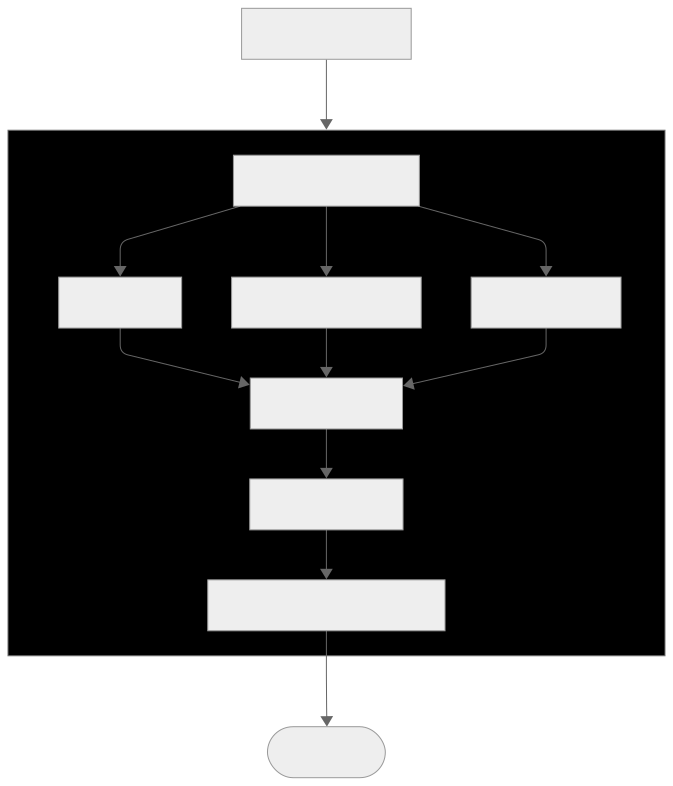
\includegraphics[width=\textwidth]{figures/loadingphase1.pdf}}
    \caption{The Loader Creation phase diagram}
    \label{fig:loadingphase1}
\end{figure}


Upon completion of the loader creation phase, a \texttt{Loader} object is produced that encapsulates the configuration 
template along with metadata about variables, constants, and execution parameters. 
\begin{minted}[fontsize=\footnotesize]{kotlin}
    interface Loader : Serializable {

    val constants: Map<String, Any?>
    val remoteDependencies: List<String>
    val launcher: Launcher
    val dependentVariables: Map<String, DependentVariable<*>>
    val variables: Map<String, Variable<*>>

    fun <T, P : Position<P>> getDefault(): Simulation<T, P>
    fun <T, P : Position<P>> getWith(values: Map<String, *>): Simulation<T, P>
    fun launch(launcher: Launcher = this.launcher): Unit
}
\end{minted}
\captionof{lstlisting}{Loader interface}

This loader serves as a factory for generating simulation instances. A Simulation can be generated by either
using the \textit{getDefault()} method, that will assign to each variable its default value, or by using the  
\textit{getWith()} method, that will assign to each variable the value provided in the map.

\paragraph{Simulation Instantiation Phase}
This phase occurs when \texttt{getDefault()} or \texttt{getWith()} is invoked with a map of variable values, that
represents the actual parameter values for that simulation instance.
So for each batch run, the getWith() method of the loader must be invoked.
This phase transforms the configuration template into an executable simulation model through the following steps:

\begin{itemize}
    \item \textbf{Variable reification}: Free variables receive their ground values from the provided map, 
    with defaults used for unspecified variables. The system validates that all provided variable names correspond 
    to known free variables.
    
    \item \textbf{Dependent variable computation}: Once all free variables have ground values, 
    dependent variables are evaluated using their registered computation functions. 
    The system ensures that all dependencies are satisfied before evaluation.
    
    \item \textbf{Simulation model construction}: The system constructs the complete simulation model, including:
    \begin{itemize}
        \item \textit{Incarnation} type of the simulation;
        \item \textit{Environment} instantiation with specified dimensions and properties;
        \item \textit{Nodes} creation and deployment according to deployment descriptors;
        \item \textit{Molecules} and concentration assignment to nodes;
        \item \textit{Reactions} and program attachment to nodes;
        \item \textit{Layers} configuration for spatial data structures;
        \item \textit{Linking rules} establishment for network topology;
        \item \textit{Monitors} and \textit{exporters} setup for data collection;
        \item \textit{Simulation engine} initialization
    \end{itemize}
In this phase, the system uses reflection\footnote{\url{http://archive.today/3rOQX}}
 combined with an automatic \textit{context parameter injection} mechanism
to support Alchemist's arbitrary class loading capabilities.

First, the system resolves the class name specified in the configuration by scanning the classpath, 
allowing users to refer to classes by their simple name if unambiguous.
Then, it instantiates the class using a dependency injection strategy:
the user provides only the parameters that define the specific configuration of the object,
while the system automatically injects contextual dependencies, such as the simulation environment, 
the random number generator, or the time distribution, if they are required by the selected constructor.
This is achieved by filtering out constructor parameters that match the types of available singletons in the loading context.
Consequently, these parameters do not need to be explicitly
defined in the configuration, reducing verbosity and decoupling the configuration from 
the internal wiring of the simulation components. 
\end{itemize}

\begin{figure}[H]
    \makebox[\textwidth][c]{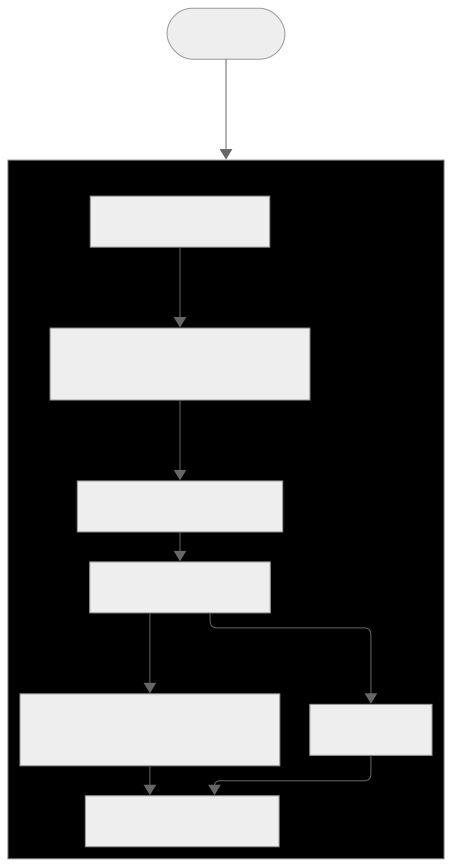
\includegraphics[width=0.4\textwidth]{figures/loadingphase2.pdf}}
    \caption{The Simulation Instantiation phase diagram}
    \label{fig:loadingphase2}
\end{figure}


This \textit{two-phase} loading system architecture provides several advantages:
\begin{enumerate}
    \item \textbf{Efficient batch execution}: a single loader can generate multiple simulation instances with different parameter
    combinations without re-parsing the configuration. 
    \item \textbf{Parameter space exploration}: by using custom launchers, the user can systematically vary 
    free variables across simulation runs.
    \item \textbf{Maintainability and extensibility}: the separation of concerns between configuration management 
    and simulation construction improves maintainability and extensibility.
\end{enumerate}

\subsection{Legacy Type System Limitations}

The Alchemist simulation model was designed to be generic over two fundamental types that define the nature of the simulated system:
\begin{itemize}
    \item \textbf{T (Concentration Type)}: Represents the type of data stored inside the nodes (molecules' concentration).
     This is defined by the specific \textit{Incarnation} used (e.g., \texttt{Double} for chemical simulations, 
     \texttt{Any} for aggregate computing).
    \item \textbf{P (Position Type)}: Represents the type of spatial coordinates used in the environment.
     This type must extend the \texttt{Position<P>} interface (e.g., \texttt{Euclidean2DPosition}, \texttt{GeoPosition}).
\end{itemize}

A fully type-safe simulation definition should theoretically propagate these two types, \texttt{<$T, P$>}, 
across all components: the \texttt{Environment}, \texttt{Nodes}, \texttt{Reactions}, and \texttt{Deployments} 
should all be parameterized consistently with the simulation's incarnation.
However, the legacy codebase presents some limitations in how these generics are handled,
 creating impedance mismatches for a statically typed DSL.

\subsubsection{Generic Type Erasure in Components}
Many existing Alchemist components were not designed with full generic propagation in mind. 
The crucial limitation lies in the class definitions themselves: rather than being generic classes that propagate the \texttt{T} and \texttt{P} types (e.g., \texttt{class Grid<P> : Deployment<P>}),
 many legacy components are non-generic and implement interfaces with \textbf{star-projections} (e.g., \texttt{Deployment<Position<*>>}).
This effectively erases the connection between the component and the specific types used in the simulation.

For instance, the \texttt{Grid} deployment class implements a star-projected interface: 

\begin{minted}[fontsize=\footnotesize]{kotlin}
open class Grid
constructor(
    private val environment: Environment<*, *>,
    private val randomGenerator: RandomGenerator,
    ... // other parameters
) : Deployment<Position<*>> 
\end{minted}

Passing a specific \texttt{Environment<T, P>} to this constructor is allowed because \texttt{Environment} is covariant (or the wildcard \texttt{<*, *>} accepts any projection).
The fundamental issue arises from the interface implemented by the class: \texttt{Deployment<Position<*>>}.
A type-safe DSL for a simulation with position type \texttt{P} requires Deployments of type \texttt{Deployment<P>}.
However, \texttt{Deployment<Position<*>>} is not a subtype of \texttt{Deployment<P>}.
Even if the \texttt{Grid} instance actually generates positions compatible with \texttt{P} (because it was initialized with an environment of type \texttt{P}), 
the type system cannot verify this relationship statically due to the erased type in the return interface.

To provide a seamless user experience, the DSL must bridge this gap. 
It should prevent the user from having to perform manual casts in their configuration scripts.
Consequently, the DSL implementation acts as an adapter layer that internally handles these type mismatches, often necessitating \textbf{unchecked casts} at runtime. 
This design choice explicitly sacrifices strict compile-time safety at the internal boundary to preserve the usability of the public API.

\subsubsection{The Loader Interface Limitation}
A similar limitation exists within the \texttt{Loader} interface itself. 
As shown in the analysis of the loading system, the \texttt{Loader} interface is not generic:

\begin{minted}[fontsize=\footnotesize]{kotlin}
interface Loader : Serializable {
    // ...
    fun <T, P : Position<P>> getWith(values: Map<String, *>): Simulation<T, P>
}
\end{minted}

The \texttt{Loader} object holds the simulation template (variables, deployments, etc.) but does not carry the \texttt{<T, P>}
 type information at the class level. 
The types $T, P$ are only introduced when the \texttt{getWith} method is invoked to instantiate the simulation, 
but there is no guarantee that the method types $T, P$ are the same as the types $T, P$ of the Simulation Object.
This implies that the internal representation of the simulation components within the \texttt{Loader} effectively
erases or hides their specific generic types.
Calling the \texttt{getWith()} method with different types $T, P$ will not result in different simulation models, since
the types are determined by the internal \texttt{Incarnation}. 
If the \texttt{getWith()} invocation method types $T_1, P_1$ are different from the actual simulation types $T_2, P_2$, the runtime cast will fail.

When the DSL constructs a \texttt{Loader}, it may have compile-time knowledge of $T, P$, 
but it must package this information into a non-generic \texttt{Loader} container, losing the type information.
Later, when \texttt{getWith} is called, the system must cast a \texttt{Simulation<T, P>} from these loosely typed components.

\section{Simulation Configuration Domain}
\label{sec:domain-model}

To design a type-safe DSL that effectively replaces the YAML configuration, it is necessary to formalize the domain model of an Alchemist simulation configuration. 
While the Alchemist core meta-model (described in Chapter~\ref{sec:background}) defines the runtime entities of a simulation, the \textbf{configuration domain} focuses on the declarative structures
 required to instantiate those entities.
This domain model identifies the key concepts, their properties, and the relationships that the DSL must express.

A simulation configuration in Alchemist is not merely a description of a single system state, but rather a \textbf{template} for generating one or more simulation instances.
The domain model is composed of three distinct areas of concern:
\begin{itemize}
    \item \textbf{Variables Definition}
    \item \textbf{Execution Settings}
    \item \textbf{Model Definition}
\end{itemize}

\subsection{Variables Definition}

Alchemist supports batch execution, allowing users to define a single configuration file that produces multiple simulation runs by varying parameters.
To support this, the configuration domain distinguishes between three types of values:
\begin{itemize}
    \item \textbf{Constants}: Values that remain fixed across all batch runs.
    \item \textbf{Free Variables}: Parameters that define the design space of the experiment. 
    They do not have a single value but a range or set of values. 
    The system generates a separate simulation for each combination of free variables.
    \item \textbf{Dependent Variables}: Values computed dynamically based on the current values of free variables (using formulas).
\end{itemize}
The DSL must provide mechanisms to declare these variables and use them transparently within the configuration, 
ensuring that type safety is maintained even when values are not known until runtime.

\subsection{Execution Settings}
\label{sec:execution-settings}
This part of the domain model configures \textit{how} the simulation is executed and observed, rather than \textit{what} is simulated.
It includes:
\begin{itemize}
    \item \textbf{Launcher}: The component responsible for managing the simulation lifecycle (such as batch mode or single run mode).
    \item \textbf{Seeds}: Configuration for the pseudo-random number generators. Alchemist typically separates the \textit{scenario RNG} (used for node placement) 
    from the \textit{simulation RNG} (used for stochastic events during execution) to ensure reproducibility.
    \item \textbf{Monitors}: Observers that track the simulation progress or status (e.g., logging to console, updating a GUI).
    \item \textbf{Exporters}: Specialized components responsible for data collection. 
    They export simulation data (e.g., molecule concentrations, node positions) to external formats (e.g., CSV, databases) for further analysis.
\end{itemize}

\subsection{Model Definition}

The Model Definition describes the actual system to be simulated. 
Key entities include:

\begin{itemize}
    \item \textbf{Incarnation}: The foundational factory that defines the type system for the simulation ($T, P$). All other components must be compatible with the types defined here.
    
    \item \textbf{Environment}: Represents the spatial context of the simulation (e.g., continuous 2D space, graph, grid). It dictates the Position type \texttt{P}.
    
    \item \textbf{Network Model}: Defines the topology of connections between nodes (e.g., nodes connected if within a certain distance). This is governed by \texttt{LinkingRules}.
    
    \item \textbf{Deployments}: Declarative generators that map geometric shapes (e.g., \texttt{Grid}, \texttt{Circle}) or algorithms to spatial positions. 
    They determine where nodes are initially placed in the environment.
    
    \item \textbf{Node Templates}: Define the internal structure of nodes. Since nodes are rarely configured individually, templates describe the properties of a generic node in a deployment:
    \begin{itemize}
        \item \textbf{Contents}: Initial \texttt{Molecules} and their \texttt{Concentrations}.
        \item \textbf{Programs}: The behavioral logic, composed of \texttt{Reactions}, which in turn consist of \texttt{Conditions}, \texttt{Actions}, and a \texttt{TimeDistribution}.
    \end{itemize}
    \item \textbf{Global Programs}: Logic that operates on the entire environment rather than being attached to specific nodes. 
    Similar to node programs, they are composed of \texttt{Global Reactions} that can modify the environment.
    \item \textbf{Layers}: Scalar fields mapped over the environment (e.g., to represent temperature or pollutant distribution) that nodes can sense.
\end{itemize}
